\documentclass{article}
\usepackage[margin=1.0in]{geometry}
\usepackage{Sweave}
\begin{document}
\Sconcordance{concordance:vennDiagram.tex:vennDiagram.Rnw:%
1 2 1 1 0 37 1 1 5 2 1 1 43 1 5 5 1}

\title{SWOT Analysis of SSRI Data, Programming \& Statistics}
\maketitle
\section*{Strengths}
\begin{itemize}
  \item Familiarity with Social Science research methods and data
  \item Wide range of skills within group
  \item Skills sets overlap providing a certain amount of backup 
  \item Easy to access/hire support, especially short-term, ``tag-team'' work 
  \item Being embedded in the administrative\slash research teams builds strong working relationships with faculty, staff, students
  \item Expertise in issues related to use and management of restricted data
  \item Web Developer/Content Provider model taking hold
\end{itemize}  
\section*{Weaknesses}
\begin{itemize}
  \item Wider range of skills in a wider range of disciplines are required to tackle Social Science research questions 
  \item No clear boundaries or focus on services that should be offered 
  \item Will need more 21st century data science expertise to meet needs
  \item Coming up with appropriate, effective content for web and other media
  \item ``Gaps'' in funding are a burden on the Institute 
\end{itemize}
\section*{Challenges}
\begin{itemize}
  \item Protective (suppressive?) stance on programming services prohibits adequate marketing efforts
  \item Impact of outsourcing services is not well understood
  \item Colleges and units at PSU have fragmented and uneven access to statistical and programming (both research and administrative)  
  \item Administrative programming needs continue to grow; analytics needed  
  \item Can be difficult to collaborate with other units both inside and outside SSRI
  \item Current consultation services underused; conversely there is growing demand for statistical \emph{practitioners}
\end{itemize}

\section*{Opportunities}
\begin{itemize}
  \item Staff turnover due to retirements over next few years
  \item Research Data Center 
  \item Building relationships with other units like UL, HMC, OVPR, etc allows us to help mold their services to fit our researchers needs and provide a wider array of services efficiently  
  \item Growing recognition of the field of ``Data Science'' (usually defined as the intersection of Programming, Statistical and Substantive skills)
\end{itemize}


\begin{figure}[h]
\begin{center}
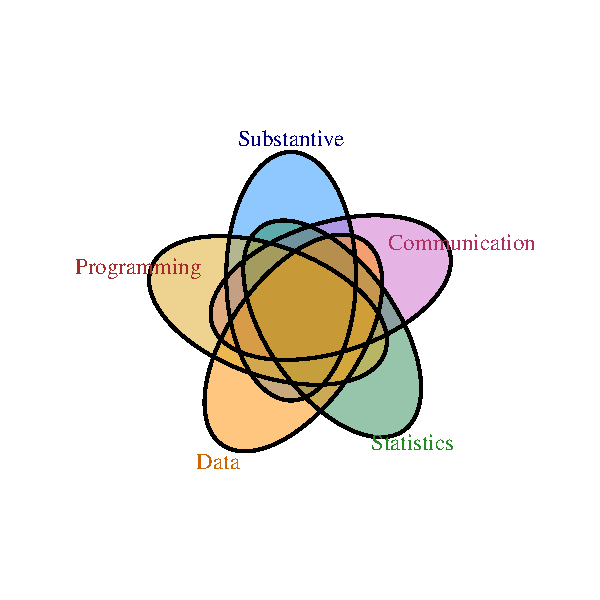
\includegraphics{vennDiagram-002}

\caption{SSRI Research Support Skill Sets}
\end{center}
\end{figure}

\end{document}
